\chapter{Model-View-* Architectures}

\section{Pendahuluan}

Model-View-* (MV*) adalah sekumpulan arsitektur yang digunakan dalam pengembangan perangkat lunak untuk memisahkan logika bisnis dari antarmuka pengguna. Pendekatan ini bertujuan untuk meningkatkan pemisahan tanggung jawab, mempermudah pengujian, serta meningkatkan keterbacaan dan pemeliharaan kode. Berbagai varian MV* meliputi \textit{Model-View-Controller} (MVC), \textit{Model-View-Presenter} (MVP), \textit{Model-View-ViewModel} (MVVM), dan \textit{Model-View-Intent} (MVI), masing-masing dengan karakteristik dan implementasi yang berbeda dalam berbagai lingkungan pengembangan.

MVC adalah pola desain yang awalnya diperkenalkan untuk mengorganisasi kode aplikasi dengan membagi tanggung jawab menjadi tiga komponen utama: \textit{Model}, yang mewakili data dan logika bisnis, \textit{View}, yang mengelola antarmuka pengguna, dan \textit{Controller}, yang bertindak sebagai mediator antara Model dan View. Seiring berkembangnya teknologi, muncul variasi MV* lainnya, seperti MVP, yang menekankan pemisahan logika presentasi dan View melalui \textit{Presenter}, MVVM, yang diperkenalkan dalam pengembangan berbasis binding data, dan MVI, yang banyak digunakan dalam pengembangan aplikasi reaktif.

Bab ini memberikan pembahasan mendalam mengenai setiap arsitektur Model-View-*, termasuk konsep dasar, perbedaan utama, keuntungan dan kerugian, serta implementasinya dalam berbagai teknologi. Contoh dunia nyata juga disajikan untuk menggambarkan bagaimana pola-pola ini diterapkan dalam pengembangan perangkat lunak modern.

\section{Model-View-Controller (MVC)}

Model-View-Controller (MVC) merupakan pola desain perangkat lunak yang memisahkan aplikasi menjadi tiga bagian utama untuk meningkatkan modularitas dan kemudahan pemeliharaan.

\subsection{MVC Klasik}

Pada implementasi klasik, MVC membagi aplikasi menjadi tiga komponen:

\begin{itemize}
	\item \textbf{Model} menangani data, logika bisnis, dan aturan bisnis aplikasi.
	\item \textbf{View} bertanggung jawab atas representasi data kepada pengguna.
	\item \textbf{Controller} menghubungkan Model dan View, menangani input pengguna, dan memperbarui Model serta View sesuai kebutuhan.
\end{itemize}

Diagram berikut menggambarkan arsitektur MVC klasik:

\begin{figure}[h]
	\centering
	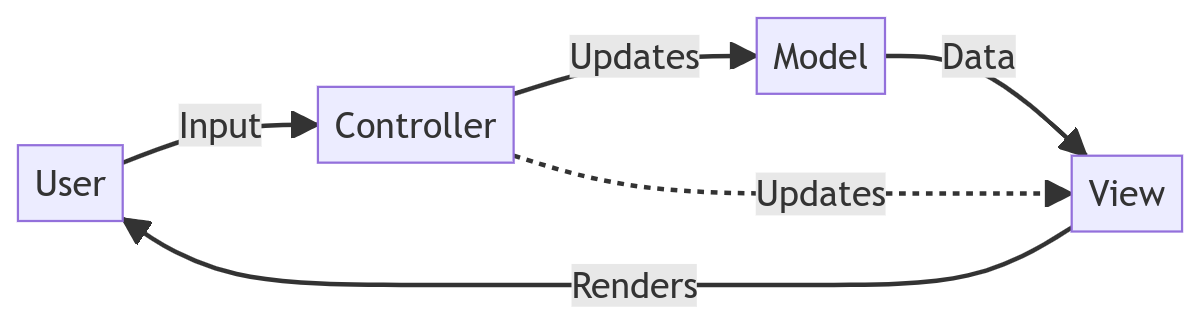
\includegraphics[width=\textwidth]{../images/mvc-classic.png}
	\caption{Classic MVC model when Users with controllers not screens}
	\label{fig:mvc-classic}
\end{figure}

\subsection{MVC dalam Kerangka Web dan Aplikasi Desktop Modern}

Banyak kerangka kerja web modern, seperti Laravel, Django, dan Spring, serta aplikasi desktop seperti JavaFX, menggunakan pendekatan MVC yang sedikit berbeda. Dalam implementasi ini:

\begin{itemize}
	\item Controller sering kali memiliki peran lebih besar, menangani logika bisnis dan interaksi dengan Model.
	\item View tidak hanya menampilkan data tetapi juga dapat berisi kode pemrograman untuk rendering dinamis.
	\item Model sering kali terintegrasi dengan ORM (\textit{Object-Relational Mapping}) untuk mempermudah akses ke basis data.
\end{itemize}

Diagram berikut menggambarkan perbedaan antara MVC klasik dan yang digunakan dalam kerangka kerja web dan aplikasi desktop modern:

\begin{figure}[h]
	\centering
	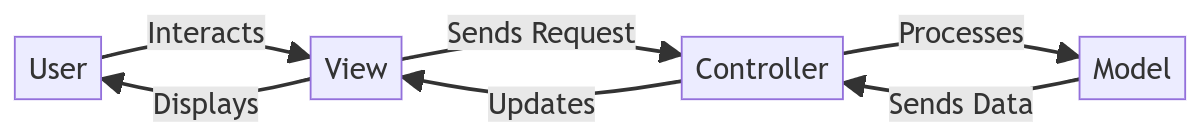
\includegraphics[width=\textwidth]{../images/mvc-modern.png}
	\caption{MVC in modern desktop/web frameworks.}
	\label{fig:mvc-modern}
\end{figure}

Pendekatan dalam kerangka kerja modern memungkinkan pemisahan lebih baik antara logika bisnis dan antarmuka pengguna, sekaligus mengintegrasikan teknologi seperti API REST dan AJAX untuk interaksi yang lebih dinamis.


\section{Model-View-Presenter (MVP)}

Model-View-Presenter (MVP) adalah pola desain yang mirip dengan MVC namun memiliki perbedaan signifikan dalam cara interaksi antara komponen-komponen tersebut. MVP lebih banyak digunakan dalam aplikasi desktop atau aplikasi yang membutuhkan pengendalian lebih besar terhadap tampilan dan interaksi pengguna. Dalam implementasi MVP:

\begin{itemize}
	\item \textbf{Model} bertanggung jawab untuk menangani logika bisnis dan data. Ini berinteraksi dengan basis data dan menyediakan data yang diperlukan oleh Presenter.
	\item \textbf{View} hanya bertugas untuk menampilkan antarmuka pengguna dan tidak mengandung logika bisnis. View akan menerima input dari pengguna dan meneruskannya ke Presenter. View bersifat pasif, artinya tidak mengelola pengolahan data atau logika bisnis.
	\item \textbf{Presenter} bertindak sebagai penghubung antara Model dan View. Presenter menerima input dari View, memprosesnya (dengan berinteraksi dengan Model), dan kemudian memperbarui View dengan data yang diperlukan.
\end{itemize}

Perbedaan utama antara \textbf{MVP} dan \textbf{MVC Klasik} terletak pada bagaimana komponen-komponen tersebut berinteraksi:
\begin{itemize}
	\item Dalam \textbf{MVP}, \textbf{Presenter} memiliki peran yang lebih besar. Semua logika bisnis dan pengolahan data dikelola oleh Presenter. View bertanggung jawab hanya untuk menampilkan data dan menerima input dari pengguna, tetapi tidak menangani pengolahan atau logika bisnis. Presenter mengelola interaksi antara Model dan View.
	\item Dalam \textbf{MVC Klasik}, \textbf{Controller} bertanggung jawab untuk menangani logika bisnis dan interaksi antara Model dan View. View hanya menampilkan data dan berinteraksi langsung dengan Controller. Dengan kata lain, Controller mempengaruhi tampilan berdasarkan aksi pengguna dengan mengubah Model, sedangkan View hanya berfungsi untuk menampilkan antarmuka pengguna.
	\item Dalam \textbf{MVP}, komunikasi antara View dan Presenter adalah dua arah, sementara dalam \textbf{MVC Klasik}, komunikasi lebih cenderung satu arah dari Controller ke View atau Model ke View.
\end{itemize}

Diagram berikut menggambarkan arsitektur MVP dan perbedaan utamanya dengan MVC Klasik:

\begin{figure}[h]
	\centering
	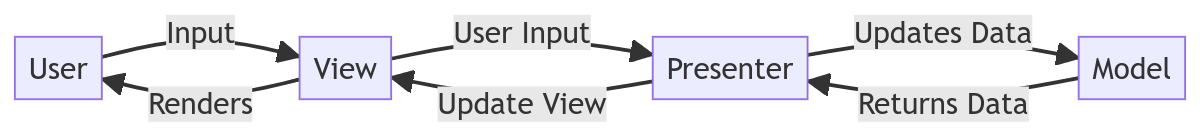
\includegraphics[width=\textwidth]{../images/mvp.png}
	\caption{Model-View-Presenter Architecture.}
	\label{fig:mvp-architecture}
\end{figure}

Keuntungan utama dari MVP adalah pemisahan yang jelas antara logika bisnis dan antarmuka pengguna, serta kemudahan pengujian unit karena Presenter dapat diuji secara terpisah tanpa bergantung pada View.

\section{Model-View-ViewModel (MVVM)}

Model-View-ViewModel (MVVM) adalah pola desain yang lebih banyak digunakan dalam aplikasi desktop dan aplikasi berbasis WPF (Windows Presentation Foundation) atau platform lain yang mendukung binding data dua arah. MVVM memisahkan logika presentasi dari antarmuka pengguna dengan cara yang sangat terstruktur. Dalam implementasi MVVM:

\begin{itemize}
	\item \textbf{Model} bertanggung jawab untuk menangani logika bisnis dan data. Model ini berinteraksi dengan basis data atau layanan lain untuk menyediakan data yang diperlukan oleh ViewModel.
	\item \textbf{View} bertanggung jawab untuk menampilkan antarmuka pengguna dan menerima input dari pengguna. View hanya berfokus pada rendering dan tidak mengelola logika atau data.
	\item \textbf{ViewModel} adalah penghubung antara View dan Model. ViewModel menangani logika presentasi, memanipulasi data yang diterima dari Model, dan menyediakan data tersebut dalam bentuk yang dapat digunakan oleh View. Dalam MVVM, ViewModel berinteraksi dengan View menggunakan binding data dua arah, yang memungkinkan pembaruan secara otomatis antara View dan ViewModel.
\end{itemize}

Perbedaan utama antara \textbf{MVVM} dan \textbf{MVP} terletak pada peran **ViewModel** dalam MVVM:
\begin{itemize}
	\item Dalam \textbf{MVVM}, \textbf{ViewModel} berfungsi untuk mempersiapkan data dari Model agar dapat digunakan oleh View. ViewModel mengelola logika presentasi dan menyediakan data dalam format yang dapat langsung dipakai oleh View.
	\item Dalam \textbf{MVP}, \textbf{Presenter} bertanggung jawab untuk memproses input dari View dan mengatur interaksi dengan Model, sementara View hanya menampilkan data dan tidak terlibat dalam pengolahan data atau logika.
	\item Dalam \textbf{MVVM}, komunikasi antara View dan ViewModel menggunakan binding data dua arah, memungkinkan pembaruan otomatis antara keduanya. Sebaliknya, dalam \textbf{MVP}, komunikasi antara View dan Presenter adalah satu arah, dimana Presenter memperbarui View dengan data yang diproses.
\end{itemize}

Diagram berikut menggambarkan arsitektur MVVM dan perbedaan utamanya dengan MVP:

\begin{figure}[h]
	\centering
	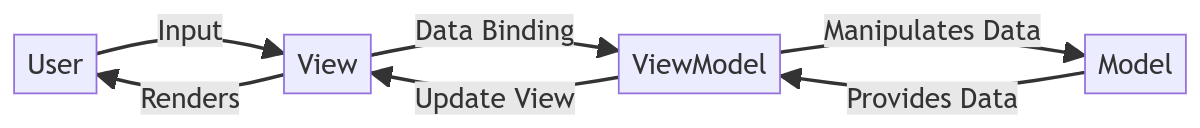
\includegraphics[width=\textwidth]{../images/mvvm.png}
	\caption{Model-View-ViewModel Architecture.}
	\label{fig:mvvm-architecture}
\end{figure}

Keuntungan utama dari MVVM adalah kemampuan untuk memisahkan logika presentasi dari antarmuka pengguna dengan menggunakan binding data dua arah, sehingga membuat pengujian dan pemeliharaan aplikasi lebih mudah. Selain itu, karena ViewModel menangani logika presentasi, View menjadi lebih sederhana dan lebih fokus pada rendering.


\section{Model-View-Intent (MVI)}

Model-View-Intent (MVI) adalah pola desain yang sering digunakan dalam aplikasi modern, terutama dalam pengembangan aplikasi Android. MVI bertujuan untuk menyederhanakan alur data dengan memberikan pendekatan yang lebih deklaratif dan reaktif. Dalam MVI, setiap komponen memiliki peran yang jelas dalam memanipulasi dan mengelola data aplikasi.

Dalam implementasi MVI:

\begin{itemize}
	\item \textbf{Model} berfungsi untuk menangani logika bisnis dan data aplikasi. Model ini menyediakan status atau keadaan aplikasi yang dapat digunakan oleh View. Model mengelola dan menyimpan data yang digunakan oleh aplikasi.
	\item \textbf{View} bertanggung jawab untuk menampilkan antarmuka pengguna dan menerima input dari pengguna. View akan mengirimkan intent ke Presenter atau ViewModel yang akan diproses lebih lanjut. View bersifat reaktif, menerima pembaruan dari Model melalui observasi data.
	\item \textbf{Intent} adalah tindakan atau niat yang dilakukan oleh pengguna yang kemudian diteruskan ke Presenter atau ViewModel untuk diproses. Intent menggambarkan apa yang ingin dilakukan oleh pengguna (misalnya, tombol ditekan atau elemen lainnya dipilih). Intent digunakan untuk memicu perubahan status pada Model atau memulai proses lain yang relevan.
\end{itemize}

Perbedaan utama antara \textbf{MVI} dan \textbf{MVP} terletak pada cara interaksi dan komunikasi antar komponen:
\begin{itemize}
	\item Dalam \textbf{MVI}, \textbf{Intent} menggantikan peran input pengguna yang secara langsung diteruskan ke ViewModel atau Presenter. Intent memfokuskan pada pengelolaan status aplikasi secara reaktif.
	\item Dalam \textbf{MVP}, \textbf{Presenter} bertanggung jawab untuk menangani logika presentasi dan memproses input dari View untuk memperbarui Model.
	\item Dalam \textbf{MVI}, komunikasi adalah satu arah dari Intent ke ViewModel atau Presenter, yang kemudian memodifikasi status Model dan mengirimkan pembaruan kembali ke View.
\end{itemize}

Diagram berikut menggambarkan arsitektur MVI dan perbedaannya dengan pola desain lain seperti MVP:

\begin{figure}[h]
	\centering
	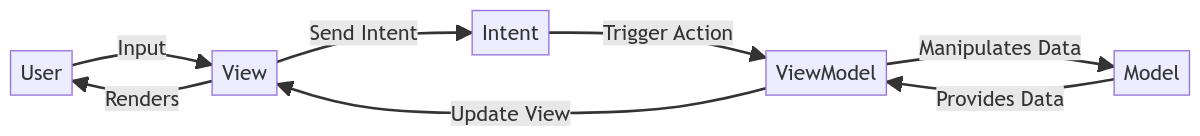
\includegraphics[width=\textwidth]{../images/mvi.png}
	\caption{Model-View-Intent Architecture.}
	\label{fig:mvi-architecture}
\end{figure}

Keuntungan utama dari MVI adalah pengelolaan status aplikasi yang lebih sederhana dan kemampuan untuk menangani alur data yang lebih reaktif. MVI juga memudahkan pemeliharaan kode dengan mengurangi kebingungan terkait interaksi antara View dan Model, serta memperkenalkan pendekatan yang lebih terstruktur untuk menangani state.


%\begin{table}[h]
%	\centering
%	\scriptsize
%	\begin{tabular}{|p{0.08\textwidth}|p{0.19\textwidth}|p{0.19\textwidth}|p{0.19\textwidth}|p{0.19\textwidth}|}
%		\hline
%		\textbf{Fitur} & \textbf{View} & \textbf{Con\-trol\-ler/\-Pre\-sent\-er/\-View\-Mo\-del} & \textbf{Model} & \textbf{Fitur Utama} \\
%		\hline
%		\textbf{MVC (Klasik)} & Menampilkan data, mengirimkan input pengguna ke Controller. & Menangani input pengguna, memperbarui View dan Model. & Menyimpan logika bisnis dan data, berinteraksi dengan basis data. & Pola klasik dengan interaksi langsung antara View, Controller, dan Model. \\
%		\hline
%		\textbf{MVC Modern} & Menampilkan data, mengirimkan input pengguna ke Controller, mungkin juga termasuk kode rendering dinamis. & Menangani input pengguna, mungkin termasuk logika tambahan, memperbarui View dan Model. & Menyimpan logika bisnis dan data, mungkin menggunakan ORM untuk pengelolaan data. & Interaksi lebih dinamis dengan logika tambahan di Controller, termasuk AJAX atau API REST. \\
%		\hline
%		\textbf{MVP} & Menampilkan data, mengirimkan input pengguna ke Presenter. & Menangani input pengguna, berinteraksi dengan Model, memperbarui View. & Menyimpan logika bisnis dan data, berinteraksi dengan basis data. & Presenter menangani seluruh logika dan pemrosesan data, \textbf{View bersifat pasif}. \\
%		\hline
%		\textbf{MVVM} & Menampilkan data, mengikat ke ViewModel menggunakan \textbf{binding data} dua arah. & Menangani logika presentasi, memanipulasi data dari Model, memperbarui View. & Menyimpan logika bisnis dan data, berinteraksi dengan basis data. & ViewModel mengikat data secara reaktif dengan View, mendukung binding data dua arah. \\
%		\hline
%		\textbf{MVI} & Menampilkan data, mengirimkan input pengguna sebagai \textbf{Intent} ke ViewModel. & Menangani pemrosesan logika, memanipulasi data dari Model, memperbarui View secara reaktif. & Menyimpan logika bisnis dan data, menyediakan pembaruan data ke ViewModel. & Pembaruan reaktif berbasis Intent, pengelolaan status disederhanakan. \\
%		\hline
%	\end{tabular}
%	\caption{Perbandingan Antara MVC (Klasik), MVC Modern, MVP, MVVM, dan MVI}
%	\label{tab:framework-comparison}
%\end{table}



%\section{Latar Belakang}
%Pada mulanya, dalam pengembangan perangkat lunak, kode yang bertanggung jawab terhadap data, logika bisnis, dan tampilan (Graphical User Interface) bercampur jadi satu, tidak ada pemisahan abstraksi.
%Pola Model-View-Controller kemudian muncul memisahkan kode program ke dalam 3 abstraksi utama berdasarkan perhatian mereka: \textit{model} untuk data, \textit{view} untuk tampilan, dan \textit{controller} untuk logika bisnis. 
%Hanya saja, MVC tidak memiliki abstraksi yang secara eksplisit mengelola \textit{states} dari tampilan (\textit{views}).
%Pola MVP (Model-View-Presenter) kemudian diajukan di mana komponen \textit{Presenter}-nya bertanggung jawab mengelola logika presentasi dari \textit{views}. Walaupun demikian,kode program yang mengelola sinkronisasi antara views dan state dari logika presentasi mereka masih harus dibuat secara manual.
%
%Keunikan dari Model-View-ViewModel adalah pola tersebut memiliki komponen \textit{binder} yang mengotomasi komunikasi/sinkronisasi antara view dengan properties yang ada pada \textit{view model}. Nilai-nilai pada \textit{view} ditautkan dengan properties pada view model sehingga perubahan nilai pada salah komponen di view (misalnya perubahan pada \textit{textbox}) akan memperbarui juga nilai pada \textit{property}-nya di \textit{view model} yang ditautkan pada komponen tersebut. Adanya binder mengurangi jumlah kode yang harus ditulis oleh developer secara manual untuk melakukan sinkronisasi antara \textit{view} dan \textit{view model}.
%
%\begin{figure}[h]
%    \centering
%    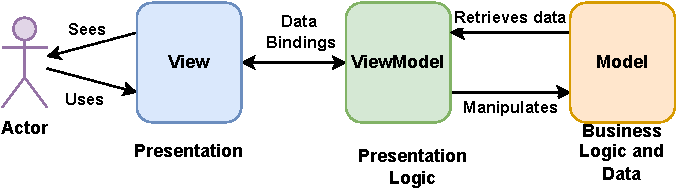
\includegraphics[width=\textwidth]{mvvm}
%    \caption{Arsitektur Model-View-ViewModel (MVVM).}
%    \label{fig:mvvm}
%\end{figure}
%
%
%\section{Arsitektur Model-View-ViewModel}
%\begin{itemize}
%\item Separation of the view layer by moving all GUI code to the view model via data binding.
%\item UI developers don't write the the GUI, instead a markup language is used.
%\item The separation of roles allows UI designers to focus on the UX design rather than programming of the business logic. 
%\item A proper separation of the view from the model is more productive, as the user interface typically changes frequently and late in the development cycle based on end-user feedback.
%\item Data bindings and properties are used to synchronise the relevant values in the view and the view model, that represents the state of the view, so that they are always the same.
%\item It eliminates or minimises application logic that directly manipulates the view. 
%
%\end{itemize}
%
%
%
%\section{Kelebihan dan Kekurangan}
%Berikut adalah kelebihan dan kekurangan arsitektur MVVM:
%
%
%\subsection{Kelebihan}
%Keuntungan dari menerapkan arsitektur MVVM adalah:
%\begin{itemize}
%\item Separation of the view layer by moving all GUI code to the view model via data binding.
%\item UI developers don't write the the GUI, instead a markup language is used.
%\item The separation of roles allows UI designers to focus on the UX design rather than programming of the business logic. 
%\item A proper separation of the view from the model is more productive, as the user interface typically changes frequently and late in the development cycle based on end-user feedback.
%\item Data bindings and properties are used to synchronise the relevant values in the view and the view model, that represents the state of the view, so that they are always the same.
%\item It eliminates or minimises application logic that directly manipulates the view. 
%
%\end{itemize}
%
%\subsection{Kekurangan}
%Konsekuensi dari penerapan arsitektur MVVM adalah sebagai berikut:
%\begin{itemize}
%\item It can be overkill for small projects. 
%\item Generalizing the viewmodel upfront can be difficult for large applications.
%\item Large-scale data binding can lead to lower performance.
%\item It's best for UI development but might not the best for other types of developments and  applications.
%\end{itemize}
%
%\section{Contoh Kasus}
%
%\subsection{Deskripsi}
%Jelaskan contoh kasus yang dipaparkan berkaitan dengan arsitektur yang dimaksud pada bab ini.
%Contoh kasus harus memperjelas arsitektur yang dimaksud.
%
%\subsection{Penjelasan Implementasi}
%Jelaskan bagian-bagian kode program, basisdata, atau konfigurasi yang signifikan terhadap arsitektur yang dimaksud.
%
%\begin{lstlisting}[firstnumber=1,style=java,caption={Model dari \textsf{Rate}.},label=lst:rate_model]
%import javax.persistence.Entity;
%import javax.persistence.Id;
%import javax.persistence.IdClass;
%
%@Entity
%@IdClass(RateId.class)
%public class Rate {
%  @Id
%  private String fromCurrency;
%  @Id
%  private String toCurrency;
%  private Double rate;
%  ...
%  Rate(String fromCurrency, String toCurrency, Double rate) {
%    ...
%  }
%  ...
%}
%\end{lstlisting}
%
%\begin{lstlisting}[firstnumber=1,style=java,caption={ \textsf{RateRepository}.},label=lst:rate_repository]
%import java.util.Collection;
%import org.springframework.data.jpa.repository.Query;
%import org.springframework.data.repository.CrudRepository;
%
%public interface RateRepository extends CrudRepository<Rate, Integer> {  
%  @Query("SELECT r FROM Rate r WHERE r.fromCurrency = ?1 and r.toCurrency = ?2")
%  Collection<Rate> findFirstByFromCurrencyAndToCurrency(String fromCurrency, String toCurrency);
%  
%  @Query("SELECT DISTINCT(r.fromCurrency) FROM Rate r")
%  Collection<String> findAllFromCurrency();
%  
%  @Query("SELECT DISTINCT(r.toCurrency) FROM Rate r")
%  Collection<String> findAllToCurrency(); 
%}
%\end{lstlisting}
%
%
%\section{Kesimpulan}
%Rangkum dan ulangi (beri penekanan pada) hal-hal kunci dari arsitektur yang dimaksud.